% =====================================================================
%  Chapter 4: Market research                     Page budget: 6 (pp. 17-22)
%  Booklet: TAM/SAM/SOM, commercial products, comparison tables,
%           performance-cost (here: price-positioning) graphs.
%  Owner: Raghad (Antigravity) - only she edits this file
% =====================================================================
\chapter{חקר שוק}
\label{ch:market}

השקת מותג קוסמטיקה חדש בשוק רווי מחייבת בסיס עובדתי מאומת לפני קבלת החלטות
אסטרטגיות. פרק זה בוחן את ההיתכנות המסחרית של מותג טינט השפתיים \en{AURA}
בישראל בשלושה רבדים משלימים: מגמות מאקרו עולמיות ומקומיות, אמידה כמותית של
היקף השוק (\en{TAM}, \en{SAM} ו-\en{SOM}), ומיפוי תחרותי של חמישה מותגים
פעילים. כל הנתונים, המחירים הקמעונאיים וערוצי הזמינות בישראל אומתו ישירות מול
דוחות שוק ואתרי מכירה רשמיים, כדי לזהות את חלל ההזדמנות שעליו נשענת בחירת
חלופת ההשקה בפרק~\ref{ch:alternatives}.

\section{מגמות מאקרו ושוק מוצרי השפתיים העולמי}
\label{sec:market-macro}

קטגוריית מוצרי השפתיים מהווה כיום אחד ממנועי הצמיחה הבולטים בענף הקוסמטיקה
העולמי. לפי מכון המחקר \en{Grand View Research}, שוק השפתונים ואיפור השפתיים
העולמי הוערך בכ-\ltr{\$17.5} מיליארד בשנת \ltr{2024}, מגיע לכ-\ltr{\$19.6}
מיליארד ב-\ltr{2026}, וצפוי לטפס עד \ltr{\$23.8} מיליארד בשנת \ltr{2030} ---
בשיעור צמיחה שנתי ממוצע (\en{CAGR}) של \ltr{4.7\%} בין השנים
\ltr{2025--2030}~\cite{grandviewresearch2025lipstick}. במקביל, שוק מוצרי טיפוח
השפתיים העולמי (\en{Lip Care Products}) הוערך בכ-\ltr{\$4.12} מיליארד בשנת
\ltr{2025}, וצפוי להגיע ל-\ltr{\$6.10} מיליארד עד שנת \ltr{2033} בקצב \en{CAGR}
גבוה אף יותר של \ltr{5.1\%}~\cite{grandviewresearch2025lipcare}.

המפגש בין שני שווקים אלה יוצר את מגמת הטיפוח-איפור ההיברידי
(\en{Skinification}): צרכניות צעירות מעדיפות טינט ושמני שפתיים המשלבים גוון
שקוף למראה טבעי (\mbox{\en{No-Makeup Look}}) עם תחושת לחות ממושכת. נתוני
\en{Circana} לשוק הביוטי היוקרתי בארה"ב ממחישים זאת היטב: בעוד קטגוריית האיפור
הכוללת צמחה ב-\ltr{5\%} ב-\ltr{2024}, קטגוריית השפתיים הובילה את הענף בזינוק
של \ltr{19\%} בהכנסות, בהובלת שמנים ובאלמים מועשרי לחות~\cite{circana2025beauty}.
מגמה זו נמשכה גם ב-\ltr{2025}, שבה שימשו מוצרי השפתיים מנוע הצמיחה המרכזי של
האיפור ותת-קטגוריית טיפולי השפתיים בעלי הגוון זינקה ביותר מ-\ltr{60\%} בחלק
מהפלחים~\cite{glossy2025lips}. לצד ההיברידיות הפונקציונלית מתחזק גל הביוטי
בהשראת מזון (\en{Food-Inspired Beauty}), שבו מותגים מובילים כגון \en{Rhode}
רותמים שמות מאכלים, ניחוחות וויזואליה עסיסית (\en{Appetite Appeal}) ליצירת
שגרת שילובי שפתיים (\en{Lip Combos}) ויראלית
ב-\en{TikTok}~\cite{voguehk2025food,glossy2025lips}.

\begin{definitionbox}[הגדרת מדדי גודל השוק]
\begin{itemize}
  \item \textbf{\en{TAM (Total Addressable Market)}:} היקף ההכנסות השנתי הכולל
    בקטגוריית הקוסמטיקה בישראל, המהווה את תקרת השוק הרחבה שבתוכה פועל המותג.
  \item \textbf{\en{SAM (Serviceable Available Market)}:} הפלח מתוך ה-\en{TAM}
    התואם לפרופיל המוצר ולקהל היעד של \en{AURA} --- סטודנטיות פעילות דיגיטלית בישראל.
  \item \textbf{\en{SOM (Serviceable Obtainable Market)}:} נתח השוק הריאלי שניתן
    לכבוש בפועל בשנה הראשונה ובתקופת ההשקה (\ltr{6} חודשים), תחת מגבלות תקציב ותחרות.
\end{itemize}
\end{definitionbox}

\section{היקף השוק בישראל ואמידת הפוטנציאל המסחרי}
\label{sec:market-sizing}

אמידת היקף השוק (\en{TAM}, \en{SAM} ו-\en{SOM}) משלבת נתון מאקרו מלמעלה למטה
(\en{Top-Down}) עם חישוב מלמטה למעלה (\en{Bottom-Up}) מנתונים דמוגרפיים רשמיים.
לפי דוח \en{Mordor Intelligence}, שוק מוצרי הקוסמטיקה בישראל מוערך
ב-\ltr{\$408.53} מיליון ב-\ltr{2026}, וצפוי להגיע ל-\ltr{\$511.64} מיליון עד
\ltr{2031} בקצב \en{CAGR} של \ltr{4.60\%}~\cite{mordor2026israel}. לפי שער
הדולר היציג סביב \ltr{3.35} ש"ח לדולר בנובמבר \ltr{2026}~\cite{boi2026rates},
עומד ה-\en{TAM} המקומי על כ-\ltr{1,369} מיליון ש"ח. מנועי הצמיחה המרכזיים
בישראל הם ריכוזיות עירונית, צמיחת מגזר היוקרה הנגישה (\en{Masstige}) והתרחבות
המסחר המקוון~\cite{mordor2026israel}. בזירה הדיגיטלית, דוח \en{Digital 2026: Israel}
של \en{DataReportal} מצביע על כ-\ltr{5.00} מיליון משתמשי \en{Instagram} בישראל
(\ltr{68.6\%} מבני \ltr{13} ומעלה) ועל כ-\ltr{4.49} מיליון משתמשי \en{TikTok}
בגיל \ltr{18} ומעלה (\ltr{69.2\%} מהבוגרים)~\cite{datareportal2026israel} ---
תשתית רחבה לפנייה ישירה לפרסונת היעד (נור, בת \ltr{22}, סטודנטית).

לגזירת ה-\en{SAM} מלמטה למעלה נעשה שימוש בנתוני ההשכלה הגבוהה הרשמיים: לפי
המועצה להשכלה גבוהה (מל"ג), בשנת תשפ"ו למדו בישראל \ltr{343,717} סטודנטים, ועם
פתיחת תשפ"ז (\ltr{2026/2027}) צפויים ללמוד כ-\ltr{350,900} סטודנטים ב-\ltr{57}
מוסדות~\cite{che2026students}. לפי הלשכה המרכזית לסטטיסטיקה (למ"ס), נשים מהוות
\ltr{60.3\%} מכלל הלומדים לתואר אקדמי~\cite{cbs2024students}, כלומר
כ-\ltr{211,600} סטודנטיות. תחת שתי הנחות עבודה שמרניות ושקופות --- אימוץ
דיגיטלי-קוסמטי של \ltr{70\%} (בהלימה לשיעורי השימוש ברשתות החברתיות,
כ-\ltr{148,100} קונות פעילות) ורכישה שנתית ממוצעת של \ltr{2.5} יחידות במחיר
היעד של \en{AURA} מתרגיל \ltr{1} (\ltr{69} ש"ח ליחידה, כלומר \ltr{172.5} ש"ח
לשנה) --- מתקבל ה-\en{SAM} השנתי של פלח הסטודנטיות:
\begin{align}
  N_{\mathheb{סטודנטיות}} &= 350{,}900 \times 0.603 \approx 211{,}593 \nonumber \\
  \text{SAM} &= 148{,}100 \times 2.5 \times 69 \approx 25.55 \times 10^6\,\mathheb{ש"ח}
  \label{eq:sam-calc}
\end{align}

עבור מותג \en{D2C} חדש, יעד חדירה ריאלי (\en{SOM}) לשנה הראשונה הוא
\ltr{1.5\%--2.5\%} מה-\en{SAM} (נקודת אמצע: \ltr{2.0\%}, כ-\ltr{2,960} לקוחות
רוכשות או כ-\ltr{7,400} יחידות מקבילות בשילוב מארזי חמשת הגוונים ב-\ltr{299}
ש"ח), המניב מחזור שנתי של כ-\ltr{511} אלף ש"ח (טווח \ltr{383--639} אלף ש"ח).
בחלון ההשקה של ששת החודשים (מכירה פעילה בחודשים \ltr{4--6}), יעד הוכחת
ההיתכנות (\en{Proof of Concept}) עומד על כ-\ltr{255} אלף ש"ח (כ-\ltr{3,700}
יחידות מקבילות). טבלה~\ref{tab:tam-sam-som} מסכמת את הנתונים, ואיור~\ref{fig:market-tam-sam-som}
מציג במשולב את תחזית הצמיחה בישראל (פאנל א') ואת משפך הסינון מן ה-\en{TAM} אל
ה-\en{SAM} וה-\en{SOM} (פאנל ב', בסקאלה לוגריתמית).

\begin{table}[htb]
  \caption{סיכום אמידת היקף השוק (\en{TAM}, \en{SAM} ו-\en{SOM}) להשקת \en{AURA} בישראל}
  \label{tab:tam-sam-som}
  \centering\auratablestripes
  \small
  \begin{tabular}{>{\raggedleft\arraybackslash}p{2.0cm} >{\raggedleft\arraybackslash}p{4.8cm} >{\raggedleft\arraybackslash}p{2.7cm} >{\raggedleft\arraybackslash}p{4.0cm}}
    \headrow \hcell{רמת שוק} & \hcell{הגדרה ושיטת חישוב} & \hcell{היקף שנתי} & \hcell{מקור / בסיס הנחה} \\
    \en{TAM} & שוק מוצרי הקוסמטיקה בישראל (\ltr{2026}), כולל איפור וטיפוח & \ltr{1,369} מיליון ש"ח (\ltr{\$408.5M}) & נתון מאומת (\en{CAGR} של \ltr{4.60\%} עד \ltr{2031})~\cite{mordor2026israel,boi2026rates} \\
    \en{SAM} & סטודנטיות פעילות דיגיטלית: \ltr{211.6K} $\times$ \ltr{70\%} $\times$ \ltr{172.5} ש"ח & \ltr{25.55} מיליון ש"ח (\ltr{\$7.63M}) & דמוגרפיה מאומתת~\cite{che2026students,cbs2024students,datareportal2026israel}; תדירות ומחיר: הנחת מודל \\
    \en{SOM} (שנה א') & חדירת יעד של \ltr{2.0\%} מה-\en{SAM} (טווח \ltr{1.5\%--2.5\%}), כ-\ltr{2,960} קונות & \ltr{0.51} מיליון ש"ח (\ltr{\$0.15M}) & יעד למותג \en{D2C} חדש; כ-\ltr{255} אלף ש"ח ב-\ltr{6} חודשי ההשקה \\
    \bottomrule
  \end{tabular}
\end{table}

\begin{figure}[htb]
  \centering
  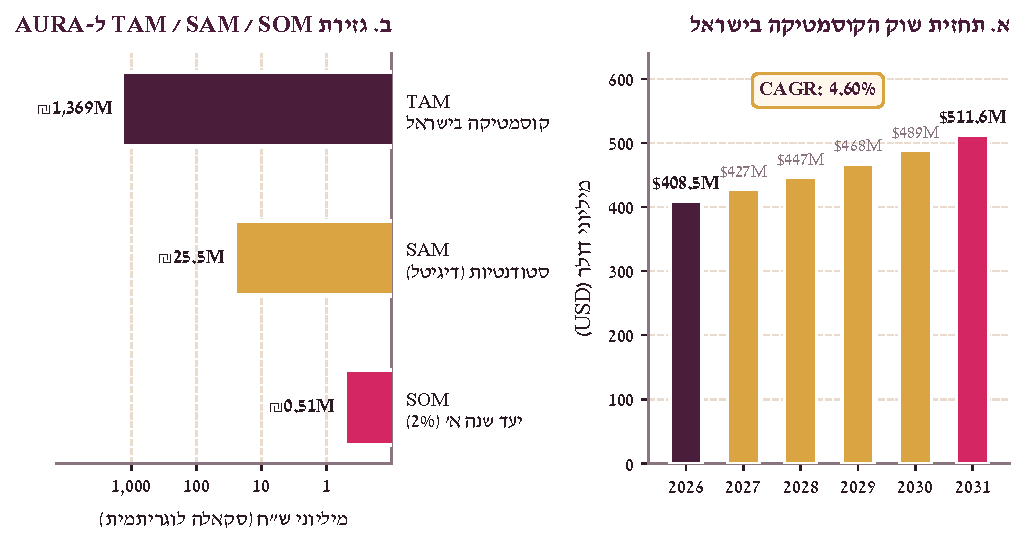
\includegraphics[width=0.95\linewidth]{market_growth_tam_sam_som.pdf}
  \caption{תחזית צמיחת שוק הקוסמטיקה בישראל (\ltr{2026--2031}) וגזירת \en{TAM},
    \en{SAM} ו-\en{SOM} עבור \en{AURA}. מקורות: \en{Mordor Intelligence}~\cite{mordor2026israel},
    מל"ג~\cite{che2026students}, למ"ס~\cite{cbs2024students} ו-\en{DataReportal}~\cite{datareportal2026israel}}
  \label{fig:market-tam-sam-som}
\end{figure}

מן הנתונים באיור~\ref{fig:market-tam-sam-som} עולה כי השוק המקומי צומח בעקביות
(תוספת של למעלה מ-\ltr{\$103} מיליון בחמש שנים), וכי יעד ה-\en{SOM} של \en{AURA}
מהווה פחות מ-\ltr{0.04\%} מכלל השוק --- יעד שמרני דיו להוכחת התאמת מוצר לשוק
(\en{Product-Market Fit}) בחמישה גווני ליבה בלבד.

\begin{insightbox}[בפרויקט שלנו: היתרון המבני של מיקוד בפרסונת ``נור'']
ריכוזן של למעלה מ-\ltr{211} אלף סטודנטיות ב-\ltr{57} קמפוסים אקדמיים, בעלות
חפיפה גבוהה בשימוש ב-\en{TikTok} וב-\en{Instagram}, מאפשר ל-\en{AURA} לשלב
קמפיין תוכן דיגיטלי עם פעילות שטח חווייתית (דוכן טעימות בקמפוס) ולהוריד את עלות
רכישת הלקוחה בהשוואה להשקה ארצית מפוזרת.
\end{insightbox}

\section{ניתוח הנוף התחרותי ומוצרים מתחרים}
\label{sec:market-competitors}

בדיקת שטח דיגיטלית מאומתת (נובמבר \ltr{2026}) מול אתרי המותגים הרשמיים ואתרי
מכירה הפעילים בישראל חשפה קיטוב חד ומפתיע בשוק טינט השפתיים המקומי. בניגוד
להערכות ראשוניות, ארבעה מתוך חמשת המותגים המוכרים ביותר סובלים מפערי מחיר או
זמינות מובהקים בישראל: \en{Rhode} (\ltr{\$20} ל-\ltr{10} מ"ל בארה"ב)
ו-\en{Rare Beauty} (\ltr{\$24} ל-\ltr{3.0} מ"ל בלבד) אינן שולחות ישירות לישראל,
ולכן מחירן אצל משווקי יבוא מקביל מקומיים מזנק ל-\ltr{155--175} ש"ח
ול-\ltr{110--140} ש"ח בהתאמה~\cite{rhode2026tint,rhode2026terms,makeupstore2026rhode,rarebeauty2026lipoil,makeupstore2026rare}.
\en{Benefit Benetint} (\ltr{\$28} ל-\ltr{6} מ"ל בארה"ב) אינו משווק באופן שוטף
בסופר-פארם או ב-\en{BE}, ונרכש בעיקר בדיוטי פרי או באתרי חו"ל בטווח
\ltr{99--125} ש"ח~\cite{benefit2026benetint,caretobeauty2026benefit}.
\en{Fenty Beauty Poutsicle} (\ltr{\$28}) אמנם שולח ישירות לישראל, אך דמי משלוח
ומסים מעלים את מחירו לכ-\ltr{130--160} ש"ח~\cite{fenty2026poutsicle,fenty2026shipping}.
מנגד, \en{Essence} זמין מיידית בסופר-פארם סביב \ltr{15} ש"ח ל-\en{What a Tint!}
(\ltr{4.9} מ"ל) ו-\ltr{6--10} ש"ח ל-\en{Juicy Bomb}~\cite{essence2026superpharm},
אך ללא ערך מותגי או נרטיב חושי. טבלה~\ref{tab:competitors} מרכזת את ההשוואה המלאה.

\begin{table}[htb]
  \caption{השוואת מתחרים מאומתת בקטגוריית טינט ושמן השפתיים בישראל (נובמבר \ltr{2026})}
  \label{tab:competitors}
  \centering\auratablestripes
  \setlength{\tabcolsep}{4pt}
  \scriptsize
  \begin{tabular}{>{\raggedleft\arraybackslash}p{2.15cm} >{\raggedleft\arraybackslash}p{2.05cm} >{\raggedleft\arraybackslash}p{1.65cm} >{\raggedleft\arraybackslash}p{1.65cm} >{\raggedleft\arraybackslash}p{2.45cm} >{\raggedleft\arraybackslash}p{3.65cm}}
    \headrow \hcell{מותג ומוצר} & \hcell{מחיר בישראל (ובארה"ב)} & \hcell{נפח ועלות למ"ל} & \hcell{מגוון גוונים} & \hcell{ערוצי מכירה וזמינות בישראל} & \hcell{מיצוב ובידול \en{AURA} מולו} \\
    \en{Rhode (Peptide Lip Tint)}~\cite{rhode2026tint,rhode2026terms,makeupstore2026rhode} &
      \ltr{155--175} ש"ח (\ltr{\$20}) &
      \ltr{10} מ"ל (\ltr{16.5} ש"ח/מ"ל) &
      \ltr{6--8} גוונים ועונתיים &
      אין משלוח ישיר; יבוא מקביל ומשלחים בלבד &
      יוקרה קרה (\en{Clean Girl}); \en{AURA} מציעה חמימות, זמינות מקומית ומחיר נגיש פי \ltr{2.4} \\
    \en{Benefit (Benetint)}~\cite{benefit2026benetint,caretobeauty2026benefit} &
      \ltr{99--125} ש"ח (\ltr{\$28} ל-\ltr{6} מ"ל) &
      \ltr{6} מ"ל (\ltr{18.7} ש"ח/מ"ל) &
      \ltr{3} גוונים (ורד, פטל, דובדבן) &
      דיוטי פרי ואתרי חו"ל; לא בסופר-פארם &
      מוצר איקוני במרקם מימי; \en{AURA} מציעה פורמולה קרמית-מלחחת ושפה עכשווית \\
    \en{Rare Beauty (Soft Pinch Oil)}~\cite{rarebeauty2026lipoil,makeupstore2026rare} &
      \ltr{110--140} ש"ח (\ltr{\$24}) &
      \ltr{3.0} מ"ל (\ltr{41.7} ש"ח/מ"ל) &
      \ltr{8} גוונים טבעיים וורודים &
      אין משלוח ישיר; בוטיקים ויבוא מקביל &
      אג'נדה רגשית-ערכית; \en{AURA} מתמקדת בעונג קולינרי ובנפח גדול פי \ltr{3.3} \\
    \en{Fenty Beauty (Poutsicle)}~\cite{fenty2026poutsicle,fenty2026shipping} &
      \ltr{130--160} ש"ח (\ltr{\$28} + משלוח) &
      \ltr{3} גר' ($\sim$\ltr{6.5} מ"ל) &
      \ltr{4--6} גוונים עזים וטרופיים &
      משלוח ישיר מהאתר עם דמי משלוח ומסים &
      נועז ועשיר בפיגמנט; \en{AURA} מותאמת למראה טבעי יומיומי לקמפוס במחיר סטודנטיאלי \\
    \en{Essence (What a Tint!)}~\cite{essence2026superpharm} &
      \ltr{15} ש"ח (גלוס \ltr{6--10}) &
      \ltr{4.9} מ"ל (\ltr{3.1} ש"ח/מ"ל) &
      \ltr{1--2} גוונים בסיסיים &
      זמינות מיידית בסופר-פארם וברשתות פארם &
      מוצר דיסקאונט פונקציונלי; \en{AURA} בונה אביזר \en{Masstige} שנור גאה לצלם \\
    \textbf{\en{AURA} (יעד השקה)} &
      \textbf{\ltr{69} ש"ח (מארז \ltr{5}: \ltr{299})} &
      \textbf{\ltr{10} מ"ל (\ltr{6.9} ש"ח/מ"ל)} &
      \textbf{\ltr{5} גווני מזון טבעיים} &
      \textbf{אתר \en{D2C} ישראלי + דוכני טעימות בקמפוס} &
      \textbf{חלל הזדמנות \en{Masstige}:} שיווק חושי חם בהשראת מזון, לחות וזמינות מקומית \\
    \bottomrule
  \end{tabular}
\end{table}

בחינת טבלה~\ref{tab:competitors} חושפת שלוש קבוצות תחרות שכל אחת מהן מותירה
פער צרכני מובהק: (א) \textbf{מותגי הפרימיום הוויראליים מיבוא} (\en{Rhode},
\en{Rare Beauty}, \en{Fenty Beauty}) יוצרים נחשקות גבוהה אך מטילים על סטודנטית
ישראלית עלות של \ltr{110--175} ש"ח (עד \ltr{41.7} ש"ח למיליליטר ב-\en{Rare Beauty})
וחיכוך של משלוחים או יבוא מקביל; (ב) \textbf{מותג המסורת \en{Benefit}} נשען על
נוסטלגיה ומרקם מימי עם \ltr{3} גוונים בלבד וזמינות מדף מוגבלת בארץ; ו-(ג)
\textbf{מותגי הפארם המוזלים (\en{Essence})} פותרים את סוגיית המחיר והזמינות, אך
נעדרים הון חברתי (\en{Social Currency}) ונרטיב קולינרי המניע שיתוף אורגני
ב-\en{TikTok}.

\section{מיצוב מחיר מול ערך וזיהוי חלל ההזדמנות}
\label{sec:market-positioning}

לצורך מפת מיצוב כמותית ושקופה הוגדר \textbf{מדד ערך חושי-מותגי ונגישות} בסולם
\ltr{1--10}, כסכום ארבעה קריטריונים בעלי משקל שווה (\ltr{0--2.5} נקודות לכל אחד):
(א) \textbf{נרטיב קולינרי וטרנדיות} --- עומק השימוש בשמות מאכלים, ניחוחות
ו-\en{Appetite Appeal}; (ב) \textbf{פורמולה היברידית מלחחת} --- שילוב גוון טבעי
עם תחושת לחות קרמית לא מייבשת; (ג) \textbf{אסתטיקת אריזה והון חברתי} --- נחשקות
כ``אביזר תיק'' ופוטנציאל ויראליות (ל-\en{AURA} ניתן ציון שמרני של \ltr{1.8} לעומת
\ltr{2.5} ל-\en{Rhode}, כהכרה ריאלית בהיעדר הילת סלבריטאית בפתיחה); ו-(ד)
\textbf{נגישות מקומית ותמורה לנפח בישראל} --- רכישה ישירה, משלוח מהיר והוגנות
המחיר למיליליטר. טבלה~\ref{tab:value-index} מפרטת את הציונים, ואיור~\ref{fig:price-positioning}
ממפה את המחיר המאומת בישראל מול מדד הערך הכולל.

\begin{table}[htb]
  \caption{פירוט ניקוד מדד הערך החושי-מותגי והנגישות (\ltr{0--2.5} לכל קריטריון, סך הכול עד \ltr{10})}
  \label{tab:value-index}
  \centering\auratablestripes
  \setlength{\tabcolsep}{4pt}
  \footnotesize
  \begin{tabular}{>{\raggedleft\arraybackslash}p{3.6cm} r r r r r}
    \headrow \hcell{מותג ומוצר} & \hcell{נרטיב קולינרי} & \hcell{פורמולה מלחחת} & \hcell{הון חברתי} & \hcell{נגישות בישראל} & \hcell{ציון כולל} \\
    \en{Essence (What a Tint!)} & \ltr{0.5} & \ltr{1.0} & \ltr{0.8} & \ltr{2.5} & \ltr{4.8} \\
    \en{Benefit (Benetint)} & \ltr{0.8} & \ltr{0.8} & \ltr{2.0} & \ltr{1.2} & \ltr{4.8} \\
    \en{Rare Beauty (Soft Pinch)} & \ltr{1.0} & \ltr{2.2} & \ltr{2.3} & \ltr{1.0} & \ltr{6.5} \\
    \en{Fenty Beauty (Poutsicle)} & \ltr{1.2} & \ltr{1.8} & \ltr{2.2} & \ltr{1.4} & \ltr{6.6} \\
    \en{Rhode (Peptide Lip Tint)} & \ltr{2.4} & \ltr{2.4} & \ltr{2.5} & \ltr{0.6} & \ltr{7.9} \\
    \textbf{\en{AURA} (יעד השקה)} & \textbf{\ltr{2.4}} & \textbf{\ltr{2.2}} & \textbf{\ltr{1.8}} & \textbf{\ltr{2.4}} & \textbf{\ltr{8.8}} \\
    \bottomrule
  \end{tabular}
\end{table}

\begin{figure}[htb]
  \centering
  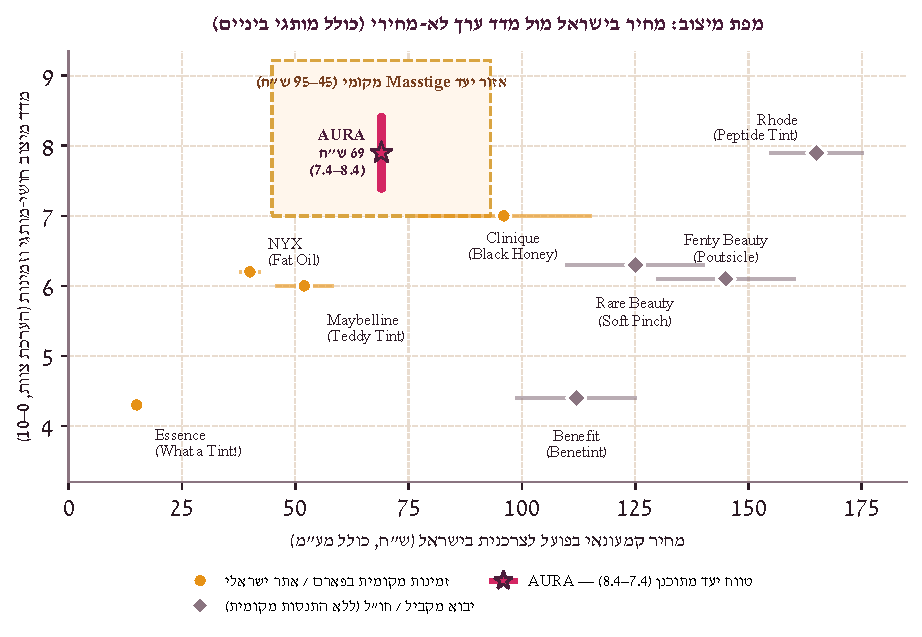
\includegraphics[width=0.86\linewidth]{price_positioning.pdf}
  \caption{מפת מיצוב: מחיר בפועל לצרכנית בישראל (עם טווחי מחיר מאומתים) מול מדד
    הערך החושי-מותגי והנגישות. האזור המוצלל מסמן את חלל ההזדמנות בקטגוריית
    ה-\en{Masstige} המקומית (\ltr{45--95} ש"ח)}
  \label{fig:price-positioning}
\end{figure}

מפת המיצוב באיור~\ref{fig:price-positioning} מציגה בבירור את ההזדמנות העסקית:
בין פלח הפארם המוזל (\ltr{10--20} ש"ח) לבין אשכול הפרימיום המיובא
(\ltr{99--175} ש"ח) פעור \textbf{חלל הזדמנות (\en{White Space}) רחב בטווח
\ltr{45--95} ש"ח}. תמחור היעד של \en{AURA} ב-\ltr{69} ש"ח ל-\ltr{10} מ"ל
(\ltr{6.9} ש"ח/מ"ל) זול בכ-\ltr{58\%} ממחיר \en{Rhode} בישראל ובכ-\ltr{45\%}
מ-\en{Rare Beauty}, ועדיין שומר על פער מיצובי ברור מעל מוצרי הפארם הזולים ---
פער חיוני לבניית דימוי \en{Masstige} איכותי ולמימון חוויית מותג עשירה. בנוסף,
העובדה שכל ארבעת מותגי הפרימיום במפה נרכשים בישראל מרחוק (מעוינים) מונעת מן
הצרכנית להתנסות בניחוח, במרקם ובגוון טרם הקנייה. ממצא זה מוביל ישירות אל
פרק~\ref{ch:alternatives}, שבו יושוו חלופות ההשקה לפי יכולתן לגשר על חסם
ההתנסות החושית תוך שמירה על יתרון המחיר המקומי.

\begin{keymessage}[המסר המרכזי מחקר השוק]
שוק הקוסמטיקה בישראל (\ltr{\$408.5} מיליון ב-\ltr{2026}, צמיחה שנתית של
\ltr{4.60\%}) וזינוק של \ltr{19\%} בקטגוריית השפתיים היוקרתית מייצרים תנאי פתיחה
נוחים ל-\en{AURA}. פערי המחיר והמשלוח של המתחרים הבינלאומיים (\ltr{99--175} ש"ח
בישראל) מותירים חלל \en{Masstige} בלתי תפוס סביב \ltr{69} ש"ח --- חלל שבו ניתן
להשיג יעד ריאלי של כ-\ltr{2\%} משוק הסטודנטיות הפעילות בשנה הראשונה (כ-\ltr{511}
אלף ש"ח) באמצעות שילוב של חמימות קולינרית, לחות וזמינות מקומית מיידית.
\end{keymessage}
